\section{Primavera}

O \textit{UnitBox} disponibiliza no \textit{Central Management} um separador que permite editar as configuração relativas aos serviços do \textit{Primavera}.

\subsection{Instalação}

Para activar o separador do \textit{Primavera} no \textit{Central Management} é necessário proceder à instalação do agente na máquina virtual.

O processo de instalação segue os seguintes passos:

\begin{figure}[H]
    \begin{center}
    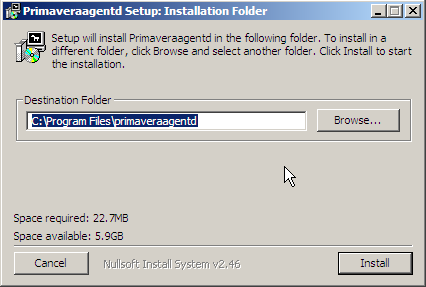
\includegraphics[scale=0.38]{screenshots/primavera/primaverainstall_01.png}
    \caption{Passo 1 - Escolha da directoria de instalação}
    \label{fig:primavera_install_passo1}
    \end{center}
\end{figure}

\begin{figure}[H]
    \begin{center}
    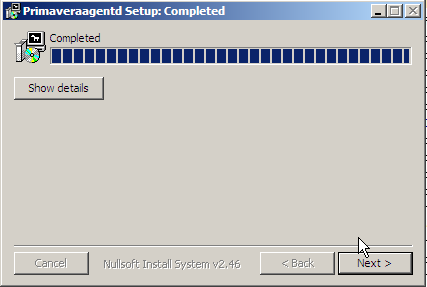
\includegraphics[scale=0.38]{screenshots/primavera/primaverainstall_02.png}
    \caption{Passo 2 - Estado da instalação}
    \label{fig:primavera_install_passo2}
    \end{center}
\end{figure}

\begin{figure}[H]
    \begin{center}
    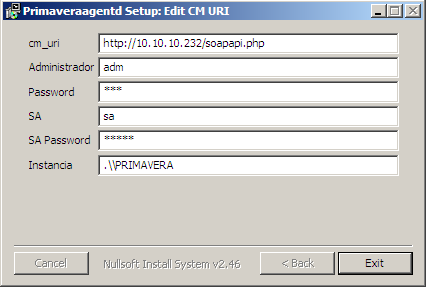
\includegraphics[scale=0.38]{screenshots/primavera/primaverainstall_03.png}
    \caption{Passo 3 - Parâmetros de configuração do Agente}
    \label{fig:primavera_install_passo3}
    \end{center}
\end{figure}

No passo 3, é necessário configurar alguns parâmetros que vão permitir aceder aos motores do \textit{Primavera} e assim permitir a sua gestão.

\begin{figure}[H]
    \begin{center}
    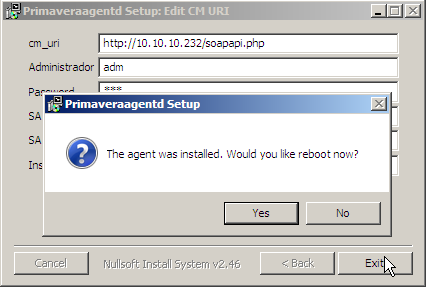
\includegraphics[scale=0.38]{screenshots/primavera/primaverainstall_04.png}
    \caption{Passo 4 - Confirmação de reboot}
    \label{fig:primavera_install_passo4}
    \end{center}
\end{figure}

\begin{figure}[H]
    \begin{center}
    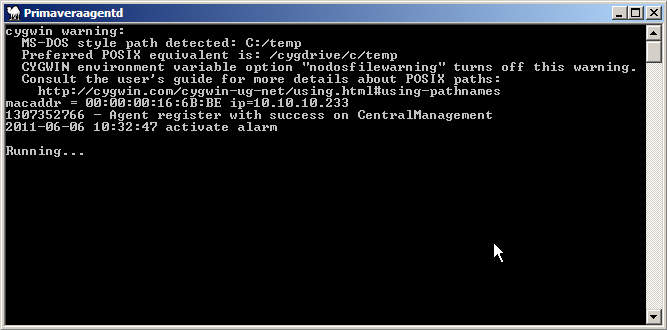
\includegraphics[scale=0.38]{screenshots/primavera/primaverainstall_05.png}
    \caption{Passo 5 - Inicialização do agente}
    \label{fig:primavera_install_passo5}
    \end{center}
\end{figure}

Após instalação é necessário proceder ao \textit{reboot} da máquina virtual para inicializar o agente.
A partir deste momento será possível a gestão do \textit{Primavera} a partir da interface do \textit{Central Mangement}.

\subsection{Interface}

A interface de gestão do \textit{Primavera} permite aceder algumas funcionalidades essenciais para a manutenção do serviço, nomeadamente, gestão de \textit{backups}, parar/arrancar serviço, gestão de utilizadores e alteração do endereço do IP da máquina virtual.

\begin{figure}[H]
    \begin{center}
    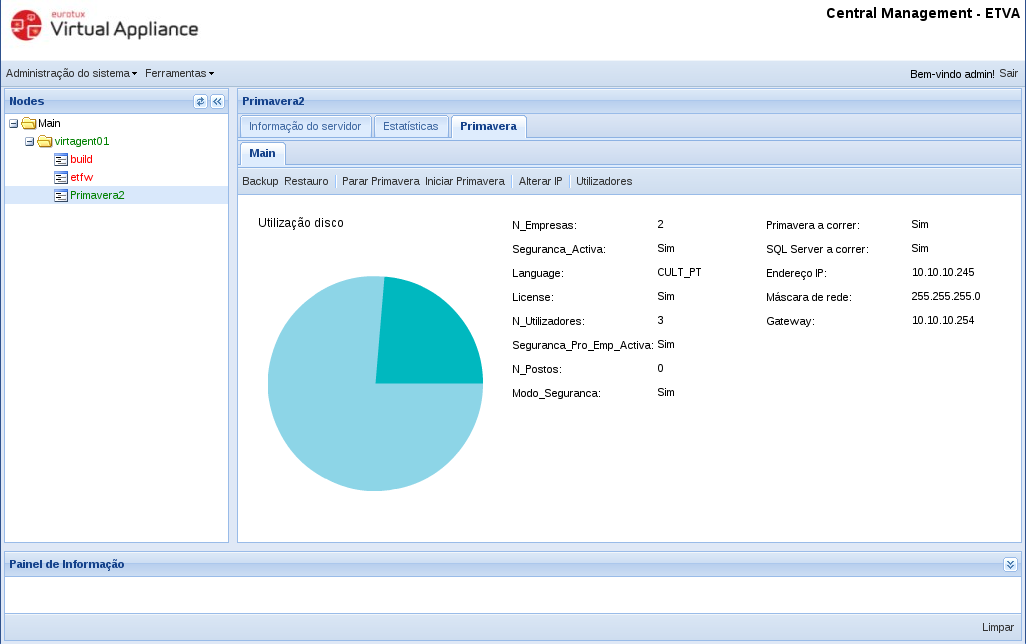
\includegraphics[scale=0.38]{screenshots/primavera/primaverainterface_01.png}
    \caption{Informação do serviço}
    \label{fig:primavera_info}
    \end{center}
\end{figure}

Logo ao aceder ao separador do \textit{Primavera} é apresentado informação relativa ao estado do serviço: utilização de espaço em disco, número de empresas, licença do \textit{Primavera}, número de postos, estado dos serviços \textit{Primavera} e \textit{SQL Server}, e informação de rede.

A partir da barra de menu é possível aceder a outras funcionalidades, nomeadamente, \textit{Backup} e restauro, parar/iniciar serviço \textit{Primavera}, alterar configuração de rede e gestão de utilizadores.

\begin{figure}[H]
    \begin{center}
    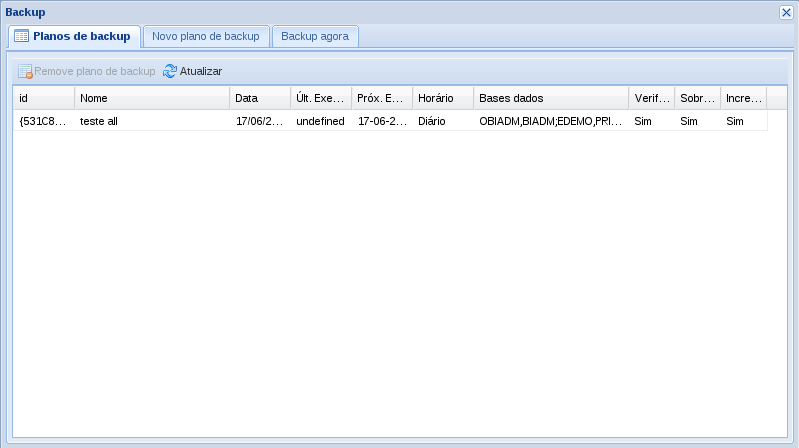
\includegraphics[scale=0.38]{screenshots/primavera/primaverainterface_02.png}
    \caption{Lista de planos de backup}
    \label{fig:primavera_list_backup_plans}
    \end{center}
\end{figure}

No menu \textit{Backup} acedemos à funcionalidade que permite gerir os planos de backup.
Para criar um novo plano de \textit{backup}, acedemos ao separador \textit{Novo plano de backup} e onde somos obrigados a definir os seguintes parâmetros: \textit{Nome} - identificação do plano, \textit{Período} - periodicidade do plano de backup (diário, semanal, mensal), \textit{Base de dados} - base de dados que serão efectuadas \textit{backup}, opções \textit{Verificar}, \textit{Sobrescrever} e \textit{Incremental}, configuram o plano para verificar após efectuar \textit{backup}, sobre-pôr o ficheiro em caso de já existir e \textit{backup} incremental.

\begin{figure}[H]
    \begin{center}
    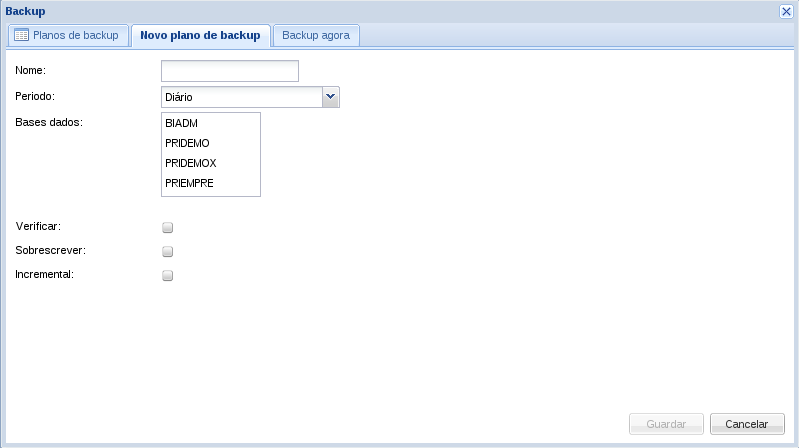
\includegraphics[scale=0.38]{screenshots/primavera/primaverainterface_03.png}
    \caption{Criar novo plano de backup}
    \label{fig:primavera_new_backup_plan}
    \end{center}
\end{figure}

\begin{figure}[H]
    \begin{center}
    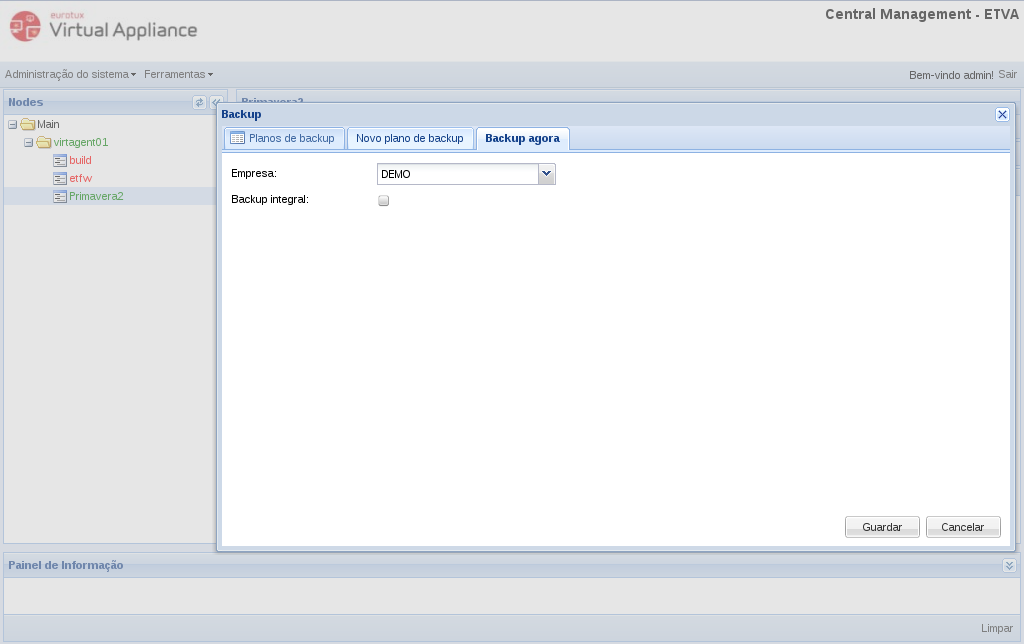
\includegraphics[scale=0.38]{screenshots/primavera/primaverainterface_04.png}
    \caption{Efectuar backup na hora}
    \label{fig:primavera_backup_now}
    \end{center}
\end{figure}

Existe ainda a opção para efectuar um \textit{backup} de imediato no separador \textit{Backup agora}. 
Aqui podemos escolher a empresa a efectuar backup ou então efectuar um \textit{backup} completo à plataforma \textit{Primavera}, escolhendo a opção \textit{Backup integral}.

\begin{figure}[H]
    \begin{center}
    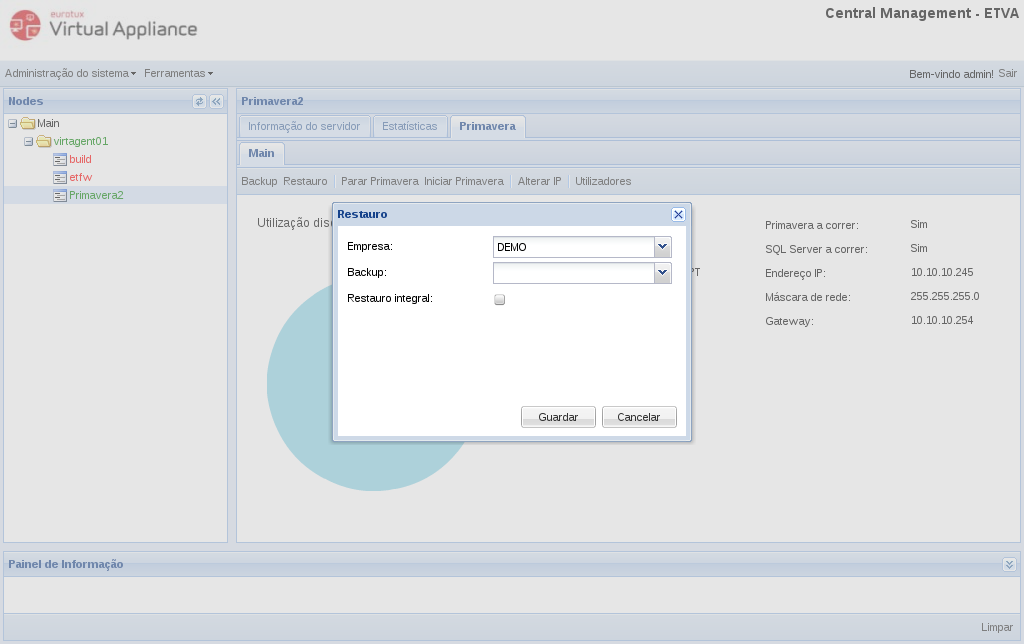
\includegraphics[scale=0.38]{screenshots/primavera/primaverainterface_05.png}
    \caption{Efectuar restauro}
    \label{fig:primavera_restore}
    \end{center}
\end{figure}

No separador de \textit{Restauro} acedemos à funcionalidade que permite repor um \textit{backup}. 
Podemos efectuar a reposição de um \textit{backup} para uma determinada empresa ou então efectuar o restauro completo do sistema com o último \textit{backup} ( opção \textit{Restauro integral} ).

\begin{figure}[H]
    \begin{center}
    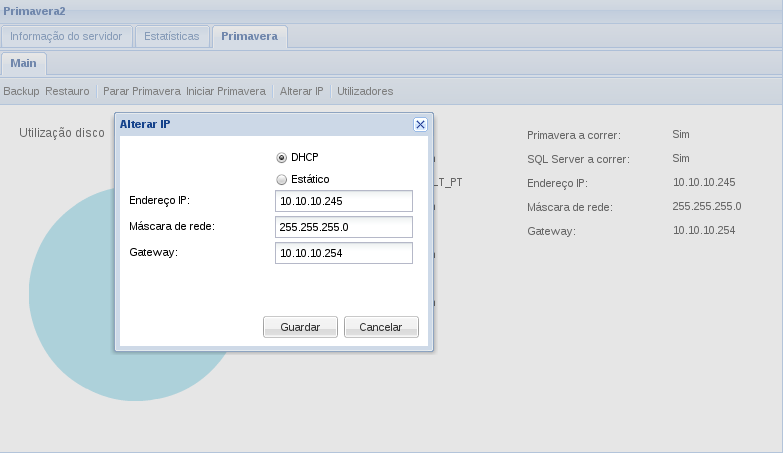
\includegraphics[scale=0.38]{screenshots/primavera/primaverainterface_06.png}
    \caption{Alterar IP}
    \label{fig:primavera_change_ip}
    \end{center}
\end{figure}

Para efectuar alteração da configuração de rede podemos aceder ao separar \textit{Alterar IP}, onde podemos modificar os parâmetros de \textit{Endereço IP}, \textit{Máscara de rede} e \textit{Gateway} da máquina virtual do \textit{Primavera}. É também possível definir que esta configuração é atribuída por \textit{DHCP}.

\begin{figure}[H]
    \begin{center}
    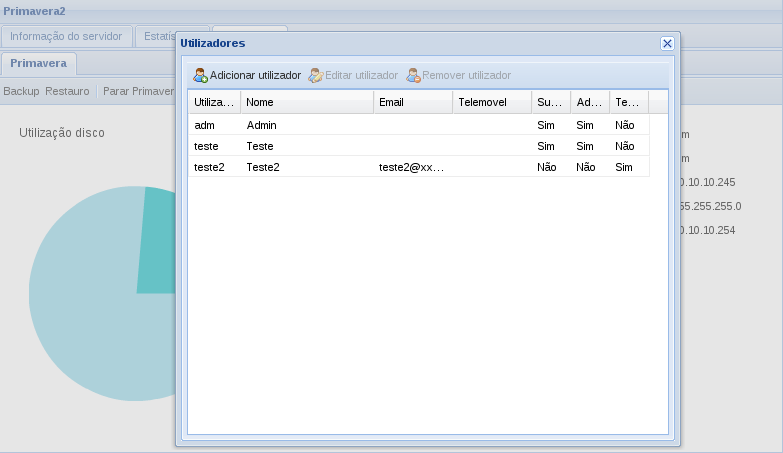
\includegraphics[scale=0.38]{screenshots/primavera/primaverainterface_07.png}
    \caption{Lista de utilizadores Primavera}
    \label{fig:primavera_list_users}
    \end{center}
\end{figure}

No separador \textit{Utilizadores} acedemos à interface de gestão dos utilizadores \textit{Primavera}.
Aqui é possível consultar os utilizadores existentes, adicionar novo utilizador com os vários parâmetros (Utilizador, Nome, Email, Password e opções Super-Administrador, Administrador e/ou Técnico ). É ainda possível editar os dados de um utilizador ou até mesmo remover do sistema.

\begin{figure}[H]
    \begin{center}
    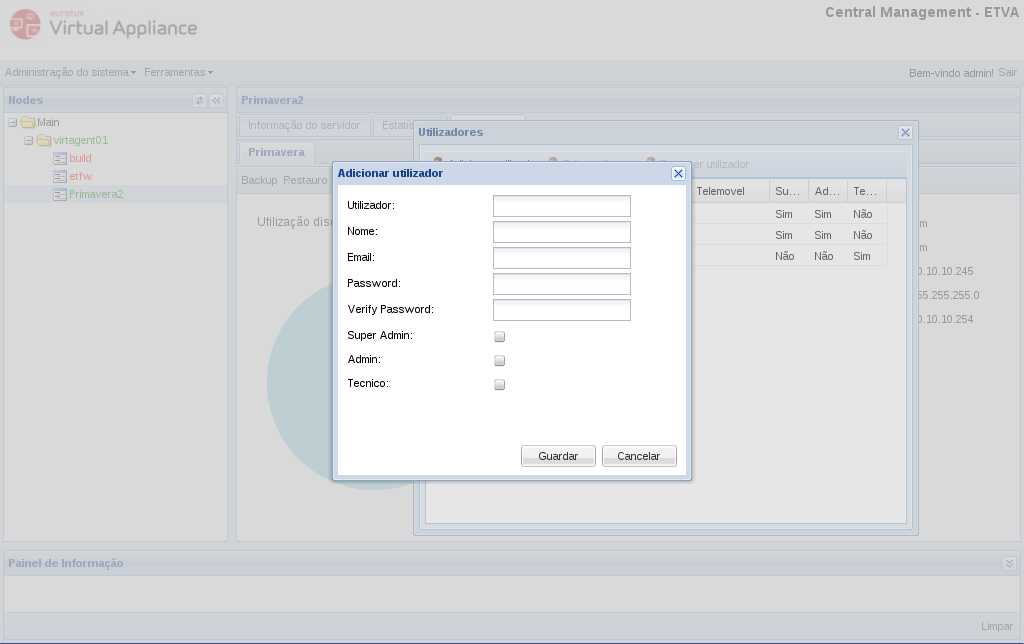
\includegraphics[scale=0.38]{screenshots/primavera/primaverainterface_08.png}
    \caption{Adicionar utilizador Primavera}
    \label{fig:primavera_add_user}
    \end{center}
\end{figure}

\begin{figure}[H]
    \begin{center}
    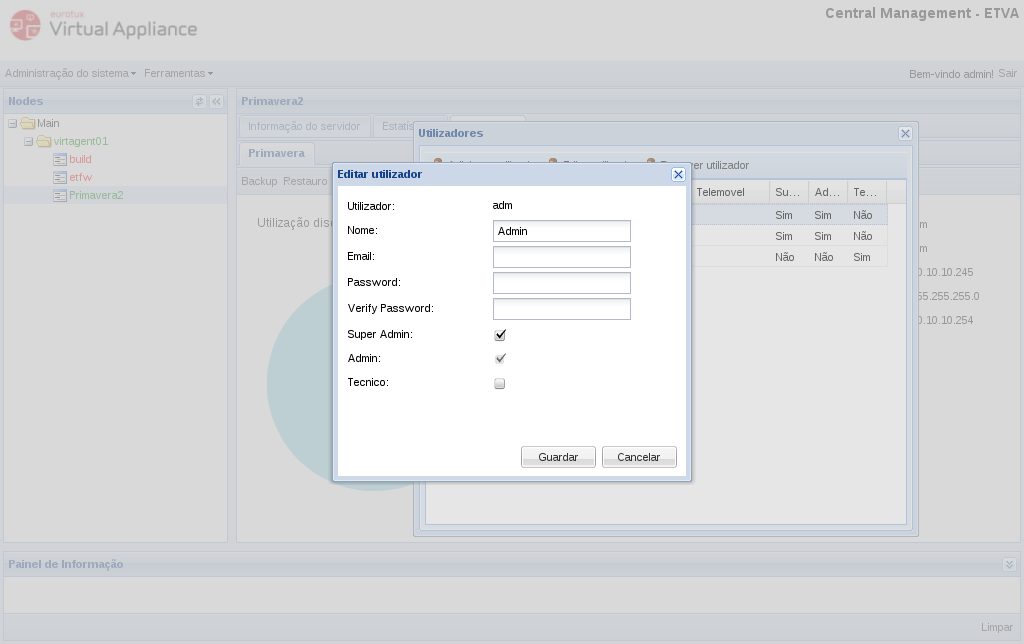
\includegraphics[scale=0.38]{screenshots/primavera/primaverainterface_09.png}
    \caption{Editar utilizador Primavera}
    \label{fig:primavera_edit_user}
    \end{center}
\end{figure}

\begin{figure}[H]
    \begin{center}
    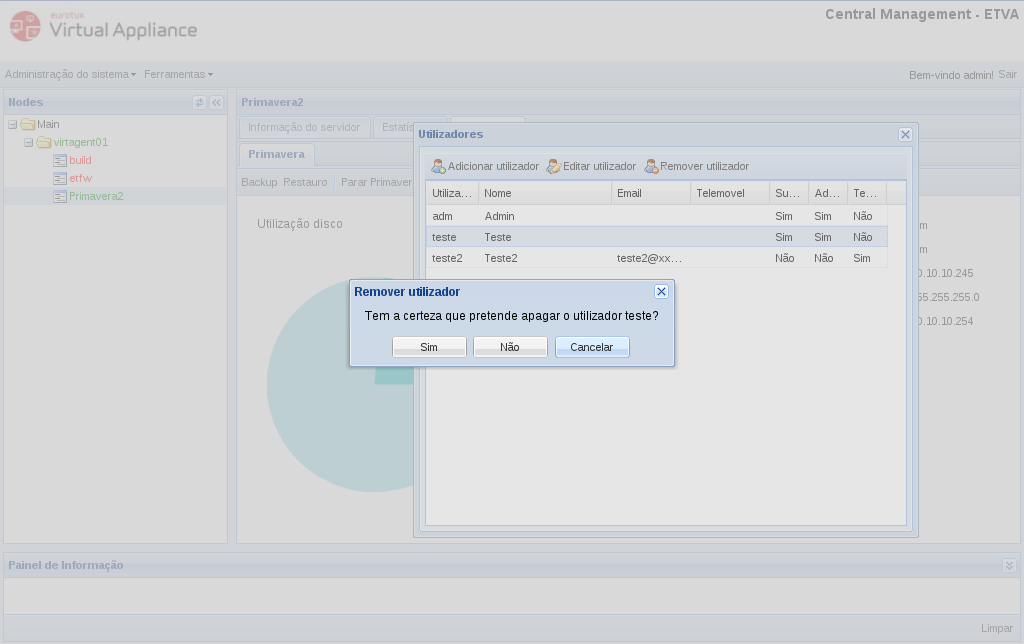
\includegraphics[scale=0.38]{screenshots/primavera/primaverainterface_10.png}
    \caption{Remover utilizador Primavera}
    \label{fig:primavera_delete_user}
    \end{center}
\end{figure}

